\chapter{Background}
%\label{cha:2}

\begin{comment}
Chapter 2: Background and literature survey
This chapter should give essential background information with references to published material in research papers, books, URLs, magazine articles and even newspapers. Expand on any references to other work that have been mentioned in Chapter 1. Refer to the notes on references (below) for the preferred way of referencing publications. The reader, stimulated by the presentation of ideas in this section, may be led to consult some or all of the referenced publications. This section will be useful for any student in a subsequent year who wishes to take the project further.
\end{comment}

\section{Existing Approaches}
\plan{Ways other people try to predict the future expenditure (in stocks etc...)}

\subsection{Finance Management}
\plan{Examples of other apps that are available, Mint.com plus the mobile ones, ensuring I highlight things they don't do}

\begin{itemize}
\item Categorising spending
\item Creating spending plans per category.
%\item View dates money came in and out in a calendar
\item Viewing money spent per category
\item Track progress of budget targets
\end{itemize}

\begin{figure}[h]
    \centering
    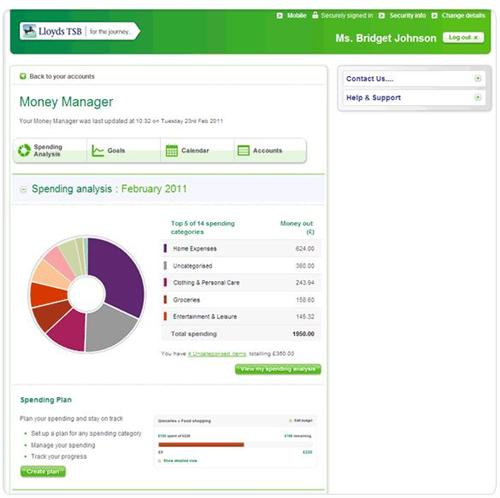
\includegraphics{moneymanagerchart}
    \caption{Spending Analysis on Money Manager \parencite{lloyds2014money}}
    \label{fig:moneymanager}
\end{figure}

\subsection{Prediction}
\plan{Papers on predicting the future}

\subsection{Security}
\plan{Paper on password entropy}


